\textbf{1-1} 入射光以入射角 $i$ 射到一不透光的表面上，入射光的能流密度为 $I$ 。设表面对光的能量反射率为 $R$ 。试求该表面单位面积所受的光压和切向力。
\vfill\newpage

\textbf{1-2} 一束强激光通过小的透明物体时，由于折射而对物体产生一定的作用力。为了对此有所理解，取一个很小的玻璃三棱镜，其顶角为 $A = \pi - 2\alpha$ ，底边长为 $2h$ ，厚度为 $\omega$ ，折射率为 $n$ ，密度为 $\rho$ 。

设该棱镜处在一束沿水平 $x$ 轴方向传播的激光之中，本题自始至终假定棱镜不发生转动，即其顶角总是对准激光束射来的方向，它的两个三角形侧面总是平行于 $xy$ 平面，底面总是平行于 $yz$ 平面，如近图1-2-1所示。周围空气的折射率取为 $n_a = 1$ ，棱镜各面均镀有防反射膜，确保不发生反射。
\begin{center}
    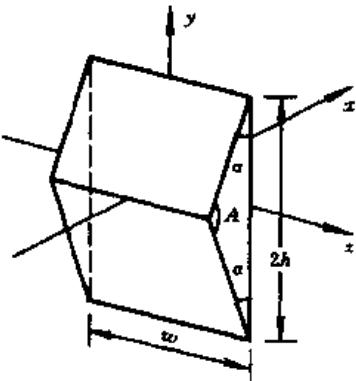
\includegraphics[width=0.2\textwidth]{figures/近图1-2-1.jpg}
    \qquad\qquad
    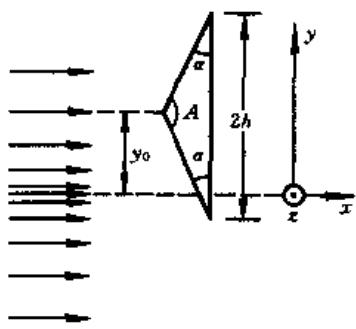
\includegraphics[width=0.2\textwidth]{figures/近图1-2-2.jpg}
    \qquad\qquad
    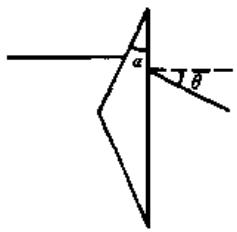
\includegraphics[width=0.2\textwidth]{figures/近图1-2-3.jpg}
\end{center}

如近图1-2-2所示，激光束的强度沿 $z$ 轴方向均匀分布，但是从 $x$ 轴开始，沿 $y$ 轴正、负方向的光强按线性关系减弱，在 $y = 0$ 处强度最大，其值为 $I_0$ ，而在 $y = \pm 4h$ 处，光强降为零。光的强度即为每单位面积的功率，单位是 $\mathbf{W} / \mathbf{m}^2$

1. 如近图 1-2-3 所示, 在激光射到棱镜上表面时, 试求偏转角 $\theta$ .

2. 将棱镜顶端由原来的位置 $x$ 轴处沿 $y$ 轴方向平移 $y_0$ , 设 $|y_0| \leqslant 3h$ . 试用 $I_0, \theta, h, w$ 和 $y_0$ 表述激光作用在棱镜上的净作用力的 $x$ 分量和 $y$ 分量. 作图表示出作用力在水平方向 ( $x$ 轴方向) 和竖直方向 ( $y$ 轴方向) 的分量随位移 $y_0$ 的变化关系.

3. 设激光束在 $z$ 方向的宽度为 $1\mathrm{mm}$ , 在 $y$ 方向的宽度为 $80\mu \mathrm{m}$ , 棱镜的参量为 $\alpha = 30^{\circ}, h = 10\mu \mathrm{m}, n = 1.5, w = 1\mathrm{mm}, \rho = 2.5\mathrm{g/cm}^{3}$ , 当棱镜的顶端位于激光束对称面以下的 $y_{0} = -\frac{h}{2} = -5\mu \mathrm{m}$ 时, 试问需要多少瓦的激光束功率才能使棱镜克服重力(指向 $-y$ 方向)的作用处于平衡状态?

4. 采用与第3问中相同的棱镜和激光束，在没有重力的条件下做实验，且设 $I_0 = 10^8\mathrm{W / m}^2$，

移动棱镜使其顶端静止地处于 $y_0 = \frac{h}{20}$ 的位置，尔后释放棱镜，它将发生振动，试求振动周期。

\vfill

\newpage
\textbf{3} 如近图1-4-1所示，一个用理想的黑色物质做成的均匀球，半径为 $r = 1\mathrm{mm}$ ，受到均匀的平行激光束的全面照射。激光是圆偏振光，波长 $\lambda = 10^{4}\mathrm{nm}$ 。球开始时在无重力的空间实验室中静止地悬浮, 经激光束照射后开始平动和转动, 球上除与激光束平行的一条直径外, 球的每一部位都沿螺旋轨道运动. 试求螺旋轨道的螺距 $h$ . 设在讨论的时间范围内, 激光束的强度不变.

注意,单色圆偏振光可以看作是一群运动光子,每个光子都带有相同的能量、相同的动量和相同的角动量,角动量矢量的方向或与动量矢量的方向平行,或反平行.对于圆偏振光,所有光子的角动量方向一致,

光子的角动量的大小为 $\pi=\frac{h}{2\pi}$ .

\begin{figure}[htbp]
\centering
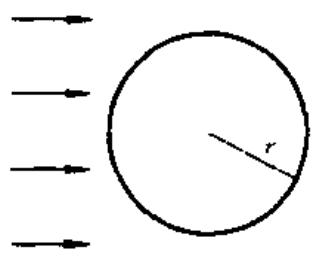
\includegraphics[width=0.6\textwidth]{figures/近图1-3-1.jpg}
\caption{近图1-3-1}
\end{figure}
\vfill

\textbf{4} 如近图1-4-1所示,两块足够大的金属平板平行放置,它们的温度维持恒定,分别为 $100^{\circ}$C 和

10$^\circ$C. 两板之间抽成真空, 并插入同样大小的两块平行板. 四块板的表面均涂黑, 因而可以看作是绝对黑体.

试求:1. 插入的两块板的温度.2. 板间的能量流与其间不插两板时能量流的比值.
\vfill

\newpage
\textbf{5} 如近图1-5-1所示，一表面涂黑的圆筒形容器，直径 $d = 5.0\mathrm{cm}$ ，高 $l = 10.0\mathrm{cm}$ ，筒内盛有液氦，其温度恰好是氦的沸点 $4.2\mathrm{K}$ 。圆筒外包有绝热材料，绝热材料与圆筒之间可能存在的空隙抽成真空。绝热材料维持在液氮温度 $77\mathrm{K}$ ，其总辐射本领是同温度下黑体总辐射本领的 $\frac{1}{2}$ 。试问每小时有多少液氦蒸发掉？假设汽化的氦气立即逸出，不考虑液氦与外界的任何气体传热与固体导热。已知液氦在 $4.2\mathrm{K}$ 时的汽化热为 $L = 2.1\times 10^{4}\mathrm{J / kg}$ 。

\begin{figure}[htbp]
\centering
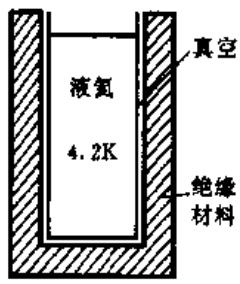
\includegraphics[width=0.6\textwidth]{figures/近图1-5-1.jpg}
\caption{近图1-5-1}
\end{figure}
\vfill

\textbf{6} 试证明在黑体的平衡辐射场中，能量密度的最大值与平衡温度 $T$ 的五次方成正比.
\vfill

\newpage
\textbf{7} 阳光中的人造卫星.

本题欲计算一颗太空中人造卫星的温度。卫星的主体假设是直径为 $1\mathrm{m}$ 的球，而且卫星主体各处温度均匀一致。卫星的整个球表面用同一种涂料覆盖。卫星处于地球附近的太空中，但不在地球的阴影中。

太阳表面温度(黑体温度) $T_{日}$ 为6000 K,太阳半径为 $R_{日}=6.96\times10^{8}m$ ,太阳与地球的距离为 $R=1.5\times10^{11}m$ .卫星在阳光中升到某一温度时,卫星的黑体辐射功率等于它对阳光的吸收功率.根据斯特藩-玻尔兹曼定律,黑体表面每单位面积的辐射功率

$$
P = \sigma T ^ {4}
$$

式中 $\sigma$ 是一普适常量, $\sigma = 5.67 \times 10^{-8} \mathrm{~W}/(\mathrm{m}^{2} \cdot \mathrm{K}^{4})$ . 我们先假设太阳与卫星都近似为黑体.

1. 试导出卫星热平衡温度 $T_{\mathrm{s}}$ 的表达式，并计算其数值。

2. 物体在温度为 T 时的黑体辐射谱 $u(T, f)$ 遵从普朗克辐射定律

$$
u (T, f) \mathrm{d} f = \frac {8 \pi k ^ {4} T ^ {4}}{c ^ {3} h ^ {3}} \cdot \frac {\eta^ {3} \mathrm{d} \eta}{\mathrm{e} ^ {\eta} - 1}
$$

式中 $udf$ 是频率在 $f$ 到 $(f + \mathrm{d}f)$ 间隔内的电磁辐射的能量密度，式中

$$
\eta = \frac {h f}{k T}
$$

有关常量如下：

$$
\begin{array}{r l} & h = 6. 6 \times 1 0 ^ {- 3 4} \mathrm{J} \cdot \mathrm{s} \\ & c = 3. 0 \times 1 0 ^ {8} \mathrm{m/s} \\ & k = 1. 4 \times 1 0 ^ {- 2 3} \mathrm{J/K} \end{array}
$$

其中 $h$ 为普朗克常量， $c$ 为真空光速， $k$ 为玻尔兹曼常量。黑体辐射谱对所有频率和发射方向进行积分，便可得到单位面积的全辐射功率 $P = \sigma T^4$ ，此即上面给出的斯特藩-玻尔兹曼定律，其中

$$
\sigma = \frac {2 \pi^ {5}}{1 5} \cdot \frac {k ^ {4}}{c ^ {2} h ^ {3}}
$$

如图所示,给出了归一化的谱(参看题后译注)

$$
\frac {k T}{h} \left[ \frac {c ^ {3} h ^ {3}}{8 \pi k ^ {4}} \cdot \frac {u (T , f)}{T ^ {4}} \right] = \frac {\eta^ {3}}{\mathrm{e} ^ {\eta} - 1}
$$

与 $\eta$ 的函数关系曲线.

在人造卫星的许多应用方面, 必须使卫星尽可能地冷. 为了冷却卫星, 工程师们使用一种反射涂料, 它可全反射掉高于某截止频率的人射光, 但是不反射低于该截止频率的热辐射. 设这一截止频率为

$$
f _ {c} = (1 2 0 0 \mathrm{K}) \frac {k}{h}
$$

试估算卫星现在可达到的温度。

不要求严格解,不必进行繁琐的积分,凡是需要的均可作近似计算.给出一个积分值如下,

$$
\int_ {0} ^ {\infty} \frac {\eta^ {3} \mathrm{d} \eta}{\mathrm{e} ^ {\eta} - 1} = \frac {\pi^ {4}}{1 5}
$$

函数 $\frac{\eta^3}{\mathrm{e}^{\eta} - 1}$ 的极大值出现在 $\eta \approx 2.82$ 处， $\eta$ 较小时，可取指数函数的近似展开式

$$
\mathrm{e} ^ {\eta} \approx 1 + \eta
$$

\begin{figure}[htbp]
\centering
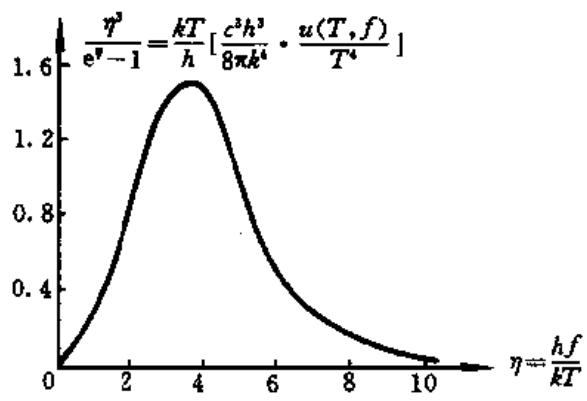
\includegraphics[width=0.6\textwidth]{figures/近图1-7-1.jpg}
\caption{近图1-7-1}
\end{figure}

3. 现在假设有一颗真实的人造卫星, 它用几块向外展开的太阳能电池板来发电, 卫星主体内电子器件的焦耳热形成了额外的热的来源. 设这种内部产生的热功率为 1KW. 试问上面第 2 问中卫星的温度又将为多少?

4. 某家厂商广告宣传一种特殊的油漆如下：''本油漆对所有人射辐射(可见光与红外线)均反射能量的90\%以上，但其本身又能像黑体一样在所有频率(可见光与红外线)上进行辐射，从而使卫星释放出的热量始终多于吸收的热量。据此，本油漆将能使卫星越来越冷。''

试问这样的油漆可能存在吗?为什么?

5. 为使一个像人造卫星一样的球体的温度上升到比第1问算出的温度还要高,试问该球表面的涂料应具有什么样的性质?
\vfill

\textbf{8} 波长为 $350\mathrm{nm}$ 的光波入射到某光电材料表面，能量最高的光电子在 $1.50\times 10^{-5}\mathrm{T}$ 的磁场中沿半径为 $18.0~\mathrm{cm}$ 的圆轨道运动。试求该光电材料的逸出功。
\vfill

\newpage
\textbf{9} 试证明,静止的自由电子不可能产生光电效应.
\vfill

\textbf{10} 在某康普顿散射实验中，散射光线与入射光线的夹角为 $60^{\circ}$ ，散射光波长为 $0.0254\mathrm{nm}$ 。试求反冲电子的动能和动量。
\vfill

\newpage
\textbf{11} 在康普顿散射中，已知反冲电子的运动方向与入射光的方向夹 $\varphi$ 角，入射光的频率为 $\nu$ ，试求反冲电子的动能。
\vfill

\textbf{12} 在一次康普顿散射中，传递给电子的最大能量为 $4.5 \times 10^{4} \mathrm{eV}$ . 试求入射光子的波长.
\vfill

\newpage
\textbf{13} 试证明，在康普顿散射中，光子的散射角 $\theta$ 与电子的散射角 $\varphi$ 之间的关系是

$$
\cot \frac {\theta}{2} = \left(1 + \frac {\lambda_ {c}}{\lambda}\right) \tan \varphi
$$

式中 $\lambda$ 是入射光的波长, $\lambda_{c}$ 是康普顿波长.
\vfill

\textbf{14} 巴耳末系中的 $\mathrm{H}_{\alpha}$ 线是指氢原子从 $n = 3$ 能级跃迁到 $n = 2$ 能级时发出的谱线，它的波长为656.280nm. 氢的同位素氘也有类似的巴耳末系，实验测得其中的 $\mathbf{D}_2$ 谱线的波长为656.101nm. 试由此确定氢核与氘核的质量比.
\vfill

\newpage
\textbf{15} 1. 试通过推导，用氢原子的玻尔半径 $R_{1}$ 和电子电量的绝对值 $\pmb{e}$ 以及真空介电常数 $\varepsilon_0$ 来表述氢原子的结合能 $\Delta E$ .

2. 设由一个 $\mu^{-}$ 子和氦核组成类氢离子, $\mu^{-}$ 的质量是电子质量的 207 倍, 其他性质与电子相同, 对于这种类氢离子, 玻尔的轨道量子化理论同样适用. 已知氢原子的 $R_{1}=0.053\ nm, \Delta E=13.6\ eV$ . 试求这种类氢离子的玻尔半径 $R'_{1}$ 和结合能 $\Delta E'$ .
\vfill

\textbf{16} 用多普勒效应测定粒子速度分布.

引言:原子发射和吸收光子是可逆过程,原子的激发及随后返回基态的过程就是一例.因此,我们可以通过观察它们吸收后的自发发射(荧光)去探测光的吸收.这种现象在探测和确定粒子以及测定粒子束速度分布的现代方法中得到运用.

在如近图1-16-1所示的理想化实验装置中，激光的波长是可变的，带一个正电荷的离子以速度 $v$ 迎着激光束的方向运动，速度 $v = 0$ 的离子可被波长 $\lambda_{1} = 600.000\mathrm{nm}$ 的激光激发。由于多普勒效应，为了激发运动离子，需要波长 $\lambda (v)$ 不同于 $\lambda_{1}$ 的激光。

\begin{figure}[htbp]
\centering
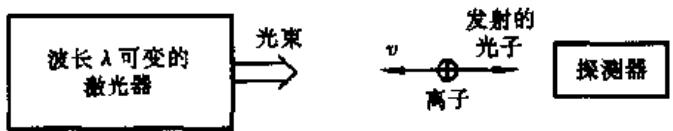
\includegraphics[width=0.6\textwidth]{figures/近图1-16-1.jpg}
\caption{近图1-16-1}
\end{figure}

设离子的数目在速度 $v_{1}=0$ 和 $v_{2}=6000\ m/s$ 的区间内均匀分布, 如近图 1-16-2 所示. 试解答以下问题.

1.(a)试问为了激发所有离子,激光的波长应在什么范围内可变?试画出受激后离子所发射的光子数按激光波长的分布曲线.

注意:在本小题中必须采用经典多普勒频移公式.

(b)上小题的严格处理需采用多普勒频移的相对论公式,即

$$
\nu^ {\prime} = \nu \sqrt {\frac {1 + \frac {v}{c}}{1 - \frac {v}{c}}}
$$

\begin{figure}[htbp]
\centering
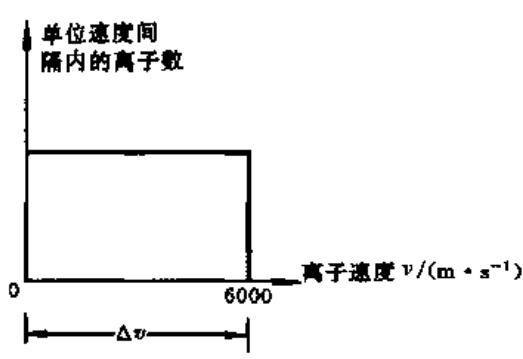
\includegraphics[width=0.6\textwidth]{figures/近图1-16-2.jpg}
\caption{近图1-16-2}
\end{figure}

试问用经典公式计算时带来的误差的数量级有多大？

2. 设离子在激发前先通过一个电势差为 $U$ 的加速电场。试求离子速度分布区间的宽度与加速电势差的定量关系。试问这个电势差使速度分布区间加宽了，还是变窄了？

3. 荷质比 $\frac{e}{m} = 4.0 \times 10^{6} \mathrm{C/kg}$ 的离子有两个激发态, 各自对应的波长为 $\lambda_{1} = 600.000 \mathrm{~nm}$ 和 $\lambda_{2} = \lambda_{1} + 10^{-3} \mathrm{~nm}$ . 试证明: 在没有加速电场的情况下要激发全部离子, 所需两组激光波长的变化范围有所重叠. 可否适当地选择一个加速电势差, 使上述两范围不重叠? 若可以, 试计算此电势差的最小值.
\vfill

\newpage
\textbf{17} 激光致冷原子.

为了能高精度地研究孤立原子的性质,必须使它们几乎静止下来并能在一个小的空间区域内停留一段时间.为此,近年来已发展成一种称为''激光致冷''的方法,其原理叙述如下.

\begin{figure}[htbp]
\centering
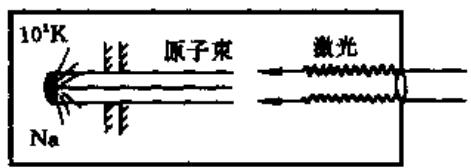
\includegraphics[width=0.6\textwidth]{figures/近图1-17-1.jpg}
\caption{近图1-17-1}
\end{figure}

\begin{figure}[htbp]
\centering
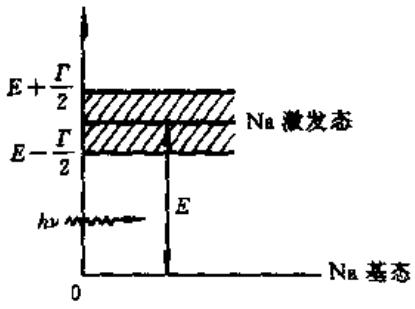
\includegraphics[width=0.6\textwidth]{figures/近图1-17-2.jpg}
\caption{近图1-17-2}
\end{figure}

在一真空室内，一束非常准直的 $\mathrm{Na}^{23}$ 原子射束（通过样品在 $10^{3}K$ 高温下蒸发而获得）受一束高强度激光的正面照射，如图 1-17-1 所示。选定激光频率，使速度为 $v_{0}$ 的钠原子可对激光光子发生共振吸收。原子吸收了光子后跃迁到能量为 E，能级宽度为 $\Gamma$ 的第一激发态，如近图 1-17-2 所示。同时它的速度有如下的改变：

$$
\Delta v _ {1} = v _ {1} - v _ {0}
$$

尔后该原子又发射光子，并再回到基态，此过程中原子的速度改变量为：

$$
\Delta \pmb {v} ^ {\prime} = \pmb {v} _ {1} ^ {\prime} - \pmb {v} _ {1}
$$

运动方向的偏转角为 $\varphi$ ，如近图1-17-3所示。这一先吸收后发射的事件可进行多次，如果不考虑偏转，把吸收和发射当作始终沿直线进行，则原子速度的总改变量达到某量 $\Delta v$ 后，便不能再对频率为 $\nu$

的激光发生共振吸收．接着需要改变激光频率，使原子在新的速度下进行共振吸收，继续减慢其速度，直到速度几乎降为零．

作为过程的第一步近似,可以忽略原子的所有其他相互作用过程,而只考虑光的吸收与再发射.进一步可以假设激光很强,所以原子在基态的停留时间实际上可以不计.

数据：

$$
\begin{array}{l l} E = 3. 3 6 \times 1 0 ^ {- 1 9} \mathrm{J} & \Gamma = 7. 0 \times 1 0 ^ {- 2 7} \mathrm{J} \\ c = 3. 0 \times 1 0 ^ {8} \mathrm{m/s} & m _ {\mathrm{p}} = 1. 6 7 \times 1 0 ^ {- 2 7} \mathrm{kg} \\ h = 6. 6 2 \times 1 0 ^ {- 3 4} \mathrm{J} \cdot \mathrm{s} & k = 1. 3 8 \times 1 0 ^ {- 2 3} \mathrm{J/K} \end{array}
$$

其中 c 为真空光速, h 为普朗克常量, k 为玻尔兹曼常量, $m_{p}$ 为质子质量.

1. 对于动能等于准直发射管后面区域内原子平均动能的那些原子,为了保证激光能被它们共振吸收,试问激光的频率 $\nu$ 须为多大? 经第一次吸收过程后,试问这些原子的速度改变量 $\Delta v_{1}$ 为多大?

2. 试问在多大速度间隔 $\Delta v_0$ 内的原子均可吸收第1问中所算出频率的光子？

3. 经过一次光子发射后, 试问原子相对发射前运动方向的最大偏转角 $\varphi_{\max}$ 为多大?

4. 若保持频率 $\nu$ 不变, 试问原子速度减少量 $\Delta v$ 至多能达到多大?

5. 为了使初速为 $v_{0}$ 沿直线运动的原子按第一问所述方式降速, 最后降到速度几乎为零, 试问需要经历吸收事件的次数 $N$ 为多少?

6. 如果一次吸收后有一次发射, 但不考虑发射引起的速度变化, 试问完成第 5 问所要求的减速过程共需多少时间? 在该时间内原子走过的路程 $\Delta s$ 为多长?
\begin{center}
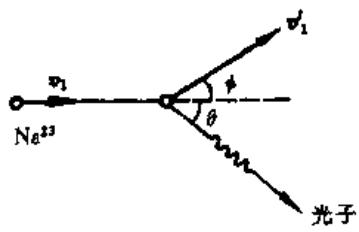
\includegraphics[width=0.3\textwidth]{figures/近图1-17-3.jpg}
\end{center}
\vfill

\textbf{18} 如近图1-18-1所示，波长为 $\lambda_0$ 的光子与一运动自由电子相碰，碰后电子静止，原光子消失, 产生一个波长为 $\lambda_{1}$ 的光子, 后者的运动方向与原光子的运动方向成 $\theta = 60^{\circ}$ 角. 之后, 此光子又与一个静止的自由电子相碰, 碰后此光子消失, 同时产生一个波长为 $\lambda_{2} = 0.125 \mathrm{~nm}$ 的光子. 后者的运动方向又与碰前光子的运动方向成 $\theta = 60^{\circ}$ 角, 如近图 1-18-2 所示. 试求第一个运动电子的德布罗意波长.

\begin{figure}[htbp]
\centering
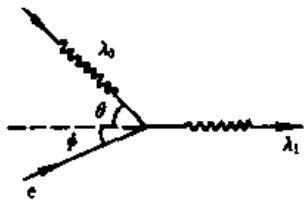
\includegraphics[width=0.6\textwidth]{figures/近图1-18-1.jpg}
\caption{近图1-18-1}
\end{figure}

\begin{figure}[htbp]
\centering
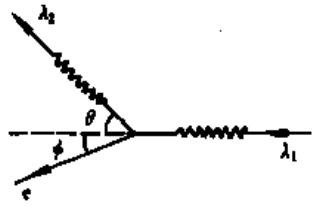
\includegraphics[width=0.6\textwidth]{figures/近图1-18-2.jpg}
\caption{近图1-18-2}
\end{figure}
\vfill

\newpage
\textbf{19} 电子束

通过加速电压 $V_{0}$ 产生一平行均匀的高能电子束。这些电子射向一条带正电荷的无限长直均匀细铜线，铜线的长度方向与电子束初始的入射方向垂直，如近图 1-19-1 所示。近图 1-19-1 中 b 表示某个电子入射方向的延长线与铜线轴线之间的距离。现在铜线带正电荷的条件下，入射电子束经铜线射向前方荧光屏的表面，屏与铜线的距离为 $L(L \gg b)$ ，如近图 1-19-1 所示。设电子束初始宽度为 $2b_{\mathrm{max}}$ ，相对铜线的轴线上下对称．在垂直于图平面方向上电子束的线度可视为无穷大.

\begin{figure}[htbp]
\centering
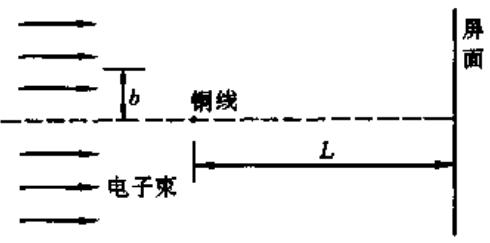
\includegraphics[width=0.6\textwidth]{figures/近图1-19-1.jpg}
\caption{近图1-19-1}
\end{figure}

有关数据如下：

铜线的半径 $r_{0}=10^{-6}$ m, b 的最大值 $b_{max}=10^{-4}$ m, 铜线每单位长度所带的电量 $q_{线密度}=4.4\times10^{-11}$ C, 给电子束加压的电压 $V_{0}=2\times10^{4}$ V, 铜线到屏面的距离 L=0.3 m.

注意:对下述第2,3,4小题,用合理的近似方法进行分析,并得出数值解答.

1. 试计算带电铜线所产生的全空间电场强度分布, 并画出电场强度大小 E 与到铜线轴之间距离的函数关系曲线.

2. 从经典物理出发，在入射的电子中对于其 $b$ 值使之不至于碰撞铜线的电子，用 $\theta_{\mathrm{e}}$ 表示它们的小偏转角，即电子入射时的初速度与到达屏面时的末速度之间的夹角。试计算 $\theta_{\mathrm{e}}$ 的值。

3. 用经典物理方法, 试粗略地确定电子束越过铜线到达屏上时在屏面上形成的图样 (即强度分布图样), 并画出图样.

4. 相对于经典物理的表述而言,量子物理对强度分布的表述有明显的区别. 试给出量子方法的定量处理步骤,并据此画出屏面上的图样.
\vfill

\textbf{20} 气体放电中的复合过程.

引言: 在足够热的气体放电中会含有各种离子. 一种离子是核电荷数为 Z 的原子被剥离到只剩下一个电子, 我们用 $A^{(Z-1)+}$ 表示这种离子. 有关数据如下:

$\varepsilon_0 = 8.854 \times 10^{-12} \mathrm{C / (V \cdot m)}$; $e$ (电子电荷) $= 1.602 \times 10^{-19} \mathrm{C}$; $q^2 = \frac{e^2}{4 \pi \varepsilon_0} = 2.307 \times 10^{-28} \mathrm{J} \cdot \mathrm{m}$ ; $\hbar = \frac{h}{2 \pi} = 1.054 \times 10^{-34} \mathrm{J} \cdot \mathrm{s}$; $m_{\mathrm{e}}$ (电子质量) $= 9.108 \times 10^{-31} \mathrm{kg}$; $r_B$ (玻尔半径) $= \frac{\hbar^2}{m_e q^2} = 5.292 \times 10^{-11} \mathrm{m}$; $E_R$ (里德伯能量) $= \frac{q^2}{2 r_B} = 2.180 \times 10^{-18} \mathrm{J}$; $m_{\mathrm{p}} C^2$ (质子静能) $= 1.503 \times 10^{-10} \mathrm{J}$ .

试解答以下五个问题.

1. 设在 $A^{(Z - 1)^+}$ 中唯一的电子处于基态, 在此态中用 $r_0^2$ 表示电子到原子核中心距离平方的平均值 (定义为位置坐标不确定量平方 $(\Delta x)^2, (\Delta y)^2, (\Delta z)^2$ 之和), 用 $p_0^2$ 表示电子动量平方的平均值 (定义为动量分量不确定量平方 $(\Delta p_x)^2, (\Delta p_y)^2, (\Delta p_z)^2$ 之和). 试问, $p_0^2$ 和 $r_0^2$ 的乘积满足什么不等式.

2. 一个 $A^{(Z - 1)+}$ 离子能俘获一个电子，并发射一个光子。试写出包含该光子角频率 $\omega_0$ 的方程组，但不必求解。

3. 利用基态能量为极小的事实, 试确定 $A^{(Z-1)+}$ 离子的基态能量. 近似条件是: 在势能表达式中用 $\frac{1}{r_0}$ 之值代替 $\frac{1}{r}$ 的平均值, $r_0$ 的值取自第 1 问. 在动能表达式中, 先用第 1 问中的 $p_0^2$ 代替动量平方的平均值, 再将第 1 问的结果表为 $p_0^2 r_0^2 = \alpha \hbar^2$ 形式, $\alpha$ 由第 1 问解答的下限确定.

4. 假设复合了的离子 $A^{(Z - 2)^+}$ 也处于基态。试用类似的方法确定该离子的能量。用 $r_1$ 和 $r_2$ （相当于第三问中的 $r_0$ ）表示两电子到原子核的平均距离，并简化地假设两电子之间的平均相对距离为 $(r_1 + r_2)$ ，再假设每个电子动量平方的平均值满足下述关系：

$$
\begin{array}{l} (p _ {1 0} ^ {2}) (r _ {1} ^ {2}) = \alpha \hbar^ {2} \\ (p _ {2 0} ^ {2}) (r _ {2} ^ {2}) = \alpha \hbar^ {2} \end{array}
$$

提示:利用基态中 $r_{1}=r_{2}$ 的事实.

5. 已知复合时发出的光子的角频率 $\omega_{0}=1.114\times10^{17}s^{-1}$ . 试求 Z 值, 试问这是什么元素的离子.

注:本小题只讨论这种特殊过程,即一个处于基态的静止离子 $A^{(Z-1)+}$ 只俘获一个静止电子.
\vfill

\newpage